
\documentclass[10pt]{article}
\usepackage[margin=1in]{geometry}
\usepackage{amsmath}
\usepackage{amssymb}
\usepackage{setspace}
\usepackage{graphicx}
\usepackage{caption}
\usepackage{subcaption} 
\usepackage{listings}


\begin{document}

\title{ECE 4750 Lab 2: Pipelined Processor}
\author{Avinash Navada (abn44) \& Akshay Dongaonkar (akd54) \& Vivek Gaddam (vrg22)}
\maketitle

\section{Introduction}

One way to improve the CPU performance over a single-cycle or FSM processor is to exploit
instruction-level parallelism (ILP) with a pipelined processor. Pipelining involves splitting up the
datapath and control into several stages using buffer registers with the potential speedup being
proportional to the number of pipeline stages. Therefore we have synthesized a 5-stage pipelined
processor that supports the PARCv2 Instruction Set Architecture (ISA). \\

We implemented a baseline pipelined design of the 5-stage pipelined processor without bypassing and an alternative, fully bypassed design. Bypassing allows for data dependencies to be resolved by using special bypass paths from the execute (X), memory access (M), and register write-back (W) stages back to the decode (D) stage. These paths allow for data dependencies to be combinationally resolved (within the same cycle), thereby eliminating the need to stall for most instructions (lw and sw are two exceptions). Therefore we expect an improvement in the transaction throughput for the bypassed design over the baseline design. 


\section{Project Management}

Changing the roles from Lab 1, we assigned Avinash to be the architect, Vivek to be the verification lead, and Akshay to be the design lead.
Our initial project roadmap was rather aggressive and required us to be finished by Sunday, September 21\textsuperscript{st}.
The Gantt Chart with both the planned and actual roadmaps overlaid is shown in Figure~\ref{fig:gantt}. Clearly, we couldn't meet the aggressive deadlines we set initially although we did manage to complete the lab before the actual deadline. \\

The work was divided as follows:
Vivek created most of the testing suite for Lab2 and worked on part of the baseline implementation.
Avinash wrote most of the writeup and created part of the testing suite.
Akshay worked on most of the baseline implementation and on the alternative implementation. 
All team members helped debug the RTL code and tests.
Akshay fixed the errors in the RTL code while Vivek and Avinash fixed the test case errors. \\

During the initial meeting on September 14, we planned to simultaneously begin the baseline implementation and the writing of directed tests the next day itself. However, various conflicts came up and we couldn't begin either of these until September 20. Akshay and Vivek worked on the baseline implementation which progressed quickly while Vivek and Avinash started the directed tests which took nearly until the end to write due to the sheer number of instructions compared to the first lab. Each test was incrementally tested on the ISA Simulator and with the baseline implementation once it was ready. All team members worked on debugging the Verilog code for the RTL implementations once the baseline implementation was done, while Vivek and Avinash debugged the test cases they worked on incrementally. We ran the 5 provided benchmarks on the baseline as well, which yielded 2 bugs that our directed tests didn't catch. Debugging the baseline was relatively straightforward since we only got 2 bugs which were resolved quickly. Once the baseline implementation was verified, Akshay began the alternative implementation which didn't take too long since adding the bypass logic and modifiying the control logic was relatively simple compared to the baseline implementation. Avinash worked on the lab report throughout this time. \\

Starting the lab earlier would have allowed us to build some extensions, although we are glad we were able to finish the assigned work on time and were able to test and evaluate our designs thoroughly. 


\section{Baseline Design}

The baseline design for this lab is a 5-stage pipelined processor with support for stalling and squashing of instructions using pipe control modules for each stage. Rather than have a state machine diagram like we did for the integer multiplier in Lab1, we have a diagram illustrating the datapath and control for the processor. \\

The baseline design was divided into datapath, control, and top-level modules due to the level of complexity. 5 Pipe control modules (one for each stage) for stall and squash signal propagation were provided to us. The interface for the baseline design consists of the following inputs: clock signal, instruction and data memory data response signals, and a manager data signal (from test source). The outputs are: instruction and data memory request and address signals, and a manager data signal (to test sink). We were initially given a basic version of the baseline implementation that supported the addu, addiu, lw, bne, and j instructions. As we incrementally added instructions, we updated the datapath and control modules accordingly to support them. \\

The last instruction we worked on implementing was the \texttt{mul} instruction. The original baseline datapath we were given did not contain a multiplier, as shown in Figure~\ref{fig:baseline}. We added our variable-latency integer multiplier from Lab 1 into this datapath, as shown in Figure~\ref{fig:baselinemult}

Two modifications we needed to add over the PARCv1 implementation discussed in lecture were sending requests/data a cycle early and implementing a val-ready interface for both instruction/data memory requests and the multiplier. The first modification was intended to save time (a cycle) by sending instruction/data memory requests at the end of the X stage instead of the beginning of the M stage so that we could get back a response from memory at the end of the M stage (assuming a one-cycle memory delay). Similarly, we could save a cycle by sending multiplier data inputs at the end of the D stage instead of the beginning of the X stage so that we get the multiplier output at the end of the X stage assuming a multiplier with a one-cycle delay. The val/ready interfaces for instruction/data memory requests and the multiplier allow for a wide range of vmemory systems and multipliers with varying latencies to be connected to the circuit. 


\section{Alternative Design}

The alternative design for this lab is a 5-stage pipelined processor with 3 bypass paths from the X, M, and W stages back to D. The only changes we made to the baseline datapath for this design were adding the bypass paths and corresponding muxes. The stall and squash signals in the control logic were also updated to account for the bypass paths. Bypass paths usually reduce the number of stall/squash signals required as data is transfered combinationally between the X/M/W stages and the D stage to resolve redundancies. The diagram of the alternative design is shown in Figure~\ref{fig:alt}. \\

We had to add an additional modification to the control module in addition to the standard changes needed to support bypassing. The control signal identifies data dependencies by checking instruction valid and register enable signals from the buffer registers at the X, M, and W stages. However, the \texttt{lw} instruction is the only instruction that is ready not at the end of the X stage but rather at the end of the M stage (after memory is read back). Hence since we also don't check the instruction when checking for data dependencies, there was no way to identify \texttt{lw} data dependencies unless we also checked for the instruction at the D stage, which is what we ended up doing. \\

One possible change we could have made to the baseline and alternative implementations is refactoring all 5 stages of the pipeline into separate modules with clearly defined interfaces to further the idea of modularity in our design. 


\section{Testing Strategy}

We began the testing process by writing and testing directed tests for all PARCv2 instructions on the ISA Simulator incrementally. Then once the baseline implementation was complete, we tested that thoroughly, and likewise for the alternative implementation. The directed tests were grouped into four categories: Basic, Bypassing, Value, and Stalls/Bubbles. The basic tests just served as guidelines for the rest of the test cases and featured 5 nops between regular instructions. The bypassing tests tested various (simple) inputs by varying numbers of nops between instructions (usually 0-5) to test various bypass paths by creating different data dependencies. The value tests focused on testing all possible input values and were further broken down into arithmetic and source/destination (testing src==dest) tests. The arithmetic tests featured a wide range of large/small/positive/negative input values, and the long tests tested stalls and bubbles by sending out a large number of instructions with data dependencies (and no nops in between) to ensure that stalls and bubbles are generated correctly and that the instructions do actually finish executing. \\

The directed test cases were made to cover all types of possible inputs, including zeros and ones, small and large numbers, positive and negative numbers, and combinations of these. The magnitude of the inputs was also varied considerably from 0 to 32 bits (even though the bit width of all the inputs is 32). Furthermore, test source/sink delays were also added to the stall/bubble (long) tests that tested the val/rdy microprotocol. The test case inputs were varied according to the instruction they were testing. A summary of all the different types of test cases is given in Table~\ref{table:tests}. \\

We only encountered two bugs with our baseline design, both of which were identified by the benchmark tests provided to us. We initially encountered a few failed directed tests, although closer inspection revealed that the issue was with incorrect test case outputs rather than with the baseline design or implementation. The first actual issue we encountered with the baseline design was with the \texttt{mul} instruction. One specific test case that issued \texttt{mfc0, mfc0,} and \texttt{mul} instructions together failed. This had to do with faulty stall logic for the \texttt{mul} instruction, which was promptly corrected. Following this, our baseline implementation failed the \texttt{vvadd-unopt} benchmark test although it passed the \texttt{vvadd-opt} test. This time the error was with the \texttt{sw} instruction stall logic. It turned out that we were not accounting for data dependencies involving the address register for the \texttt{sw} instruction (e.g. \texttt{R8} in \texttt{sw R4, 0(R8)}). After fixing this error, our baseline implementation ran successfully on all directed and benchmark tests. We did not encounter any issues with the alternative implementation, which ran correctly on all tests on the first try. \\ 

Ultimately both the base and alternative designs worked correctly with all test cases. Although there were a lot of tests covering a wide range of possible inputs for each instruction, we could have added more test cases that tested instructions streams with various combinations of instructions and types of programs. However, due to time constraints, we were not able to do so. \\


\section{Evaluation}

As soon as the base and alternative designs were completed, the next step was to test the performance of the models. In order to achieve this, the simulator harness was built and run (using the given datasets) to generate the total number of cycles and the average number of cycles per transaction for the base and alternative designs. The results of the simulator for each dataset and design are summarized in Table~\ref{tab:cycles}. \\

Analysis of evaluation results. \\


\pagebreak[4]

\section {Tables and Diagrams}

% Table: test types

\begin{center}
\begin{table}[h]
\begin{tabular}{| c | c |}
\hline
\multicolumn{2}{|c|}{Types of Directed Test Cases}   \\
\hline
\textbf{Type}                         &    \textbf{Description}  	\\   \hline      
Basic            					  &           					\\
Bypassing                             &								\\
Value: Arithmetic           		  &          					\\        
Value: Source/Destination             & 							\\
Stalls/Bypass 						  & 							\\
\hline                                                 
\end{tabular}
\caption{Types of Directed Test Cases} 
\label{table:tests}
\end{table}
\end{center}

% Table: execution cycles for evaluation

\begin{center}
\begin{table}[h]
\begin{tabular} {|l | r | r | r | r | r |}

\hline
\textbf{Design}    & \textbf{vvadd-unopt} & \textbf{vvadd-opt} & \textbf{cmplx-mult} & \textbf{bin-search} & \textbf{masked-filt} \\
\hline
Baseline:    Total Cycles                 &        &       &      & 	&						\\
Baseline:    Avg. Cycles / Transaction    &        &       &      & 	&						\\
Alternative: Total Cycles                 &        &       &      & 	&						\\
Alternative: Avg. Cycles / Transaction    &        &       &      & 	&					    \\
\hline                    
\end{tabular}
\caption{Baseline v. Alternative Design Performance}
\label{tab:cycles}
\end{table}
\end{center}

\pagebreak[4]

% Figure: Gantt Chart

\begin{figure}[b]
\centering
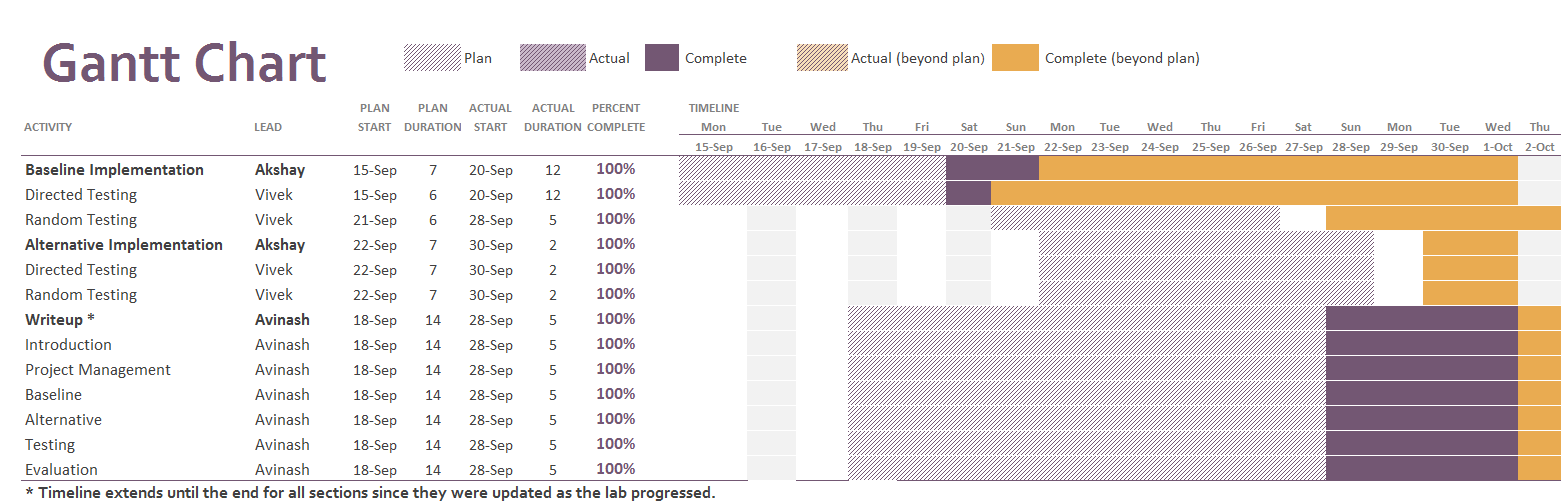
\includegraphics[scale=0.5, angle=90]{gantt}
\caption{Gantt Chart}
\label{fig:gantt}
\end{figure}


% Figure: Baseline Diagram

\begin{figure}[b]
\centering
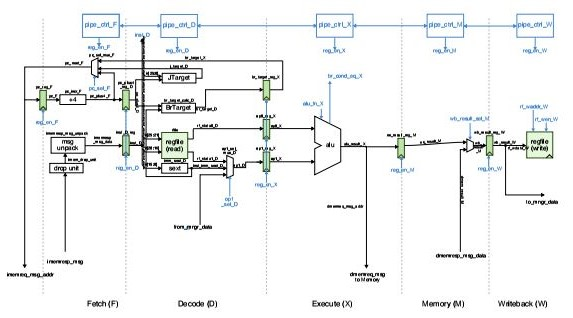
\includegraphics[scale=1.1]{baseline}
\caption{Diagram showing datapath and control of baseline 5-stage pipelined processor.}
\label{fig:baseline}
\end{figure}

% Figure: Baseline with Multiplier Diagram

\begin{figure}[b]
\centering
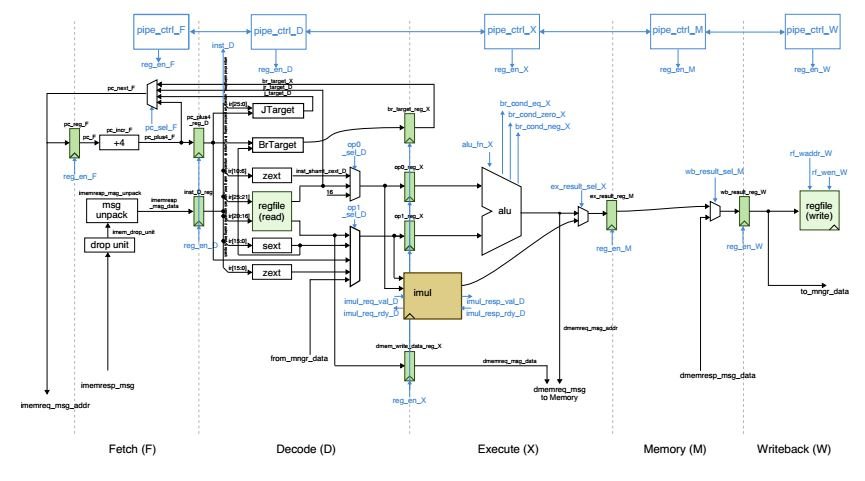
\includegraphics[scale=0.75]{baselinemult}
\caption{Diagram showing the baseline implementation with our variable-latency multiplier from Lab1.}
\label{fig:baselinemult}
\end{figure}


% Figure: Alternative Diagram

\begin{figure}[b]
\centering
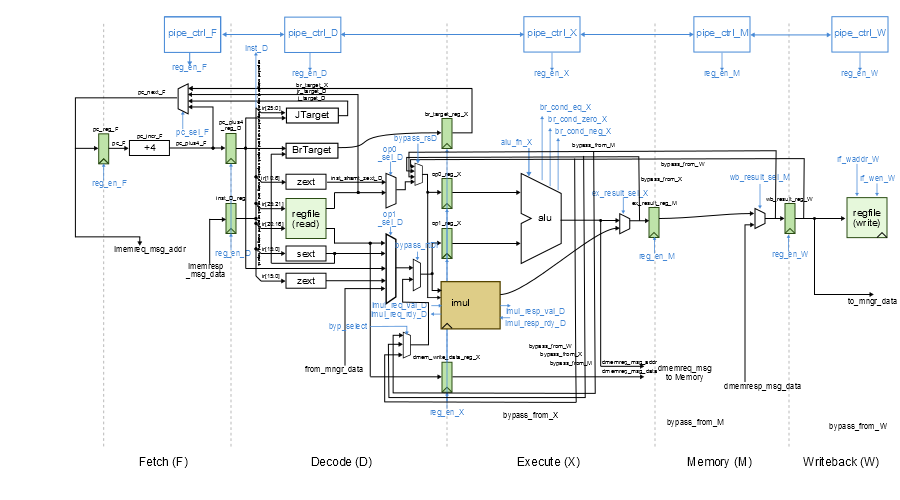
\includegraphics[scale=0.5]{alt}
\caption{Diagram showing datapath and control of alternative (fully bypassed) 5-stage pipelined processor.}
\label{fig:alternative}
\end{figure}


\end{document}
